% This is samplepaper.tex, a sample chapter demonstrating the
% LLNCS macro package for Springer Computer Science proceedings;
% Version 2.21 of 2022/01/12
%
\documentclass[runningheads]{llncs}
\bibliographystyle{splncs04}

%
\usepackage[T1]{fontenc}
% T1 fonts will be used to generate the final print and online PDFs,
% so please use T1 fonts in your manuscript whenever possible.
% Other font encondings may result in incorrect characters.
%
\usepackage{graphicx}
% Used for displaying a sample figure. If possible, figure files should
% be included in EPS format.
%
% If you use the hyperref package, please uncomment the following two lines
% to display URLs in blue roman font according to Springer's eBook style:
%\usepackage{color}
%\renewcommand\UrlFont{\color{blue}\rmfamily}
%\urlstyle{rm}
%
\begin{document}
%
\title{Techniques et outils de visualisation temporel et d'interaction avec un focus sur la réservation}
\titlerunning{Techniques et outils de visualisation temporel et d'interaction}
%
%\titlerunning{Abbreviated paper title}
% If the paper title is too long for the running head, you can set
% an abbreviated paper title here
%
\author{Merault Valentin \and
Romano Tom \and
N'Diaye Baptiste}
%
\authorrunning{Merault Valentin \and
Romano Tom \and
N'Diaye Baptiste}
% First names are abbreviated in the running head.
% If there are more than two authors, 'et al.' is used.
%
\institute{Ecole National d'Aviation Civile, France }
%
\maketitle              % typeset the header of the contribution
%
\begin{abstract}
Cet article explore les techniques et outils de visualisation des données temporelles et d'interaction utilisateur, avec un focus particulier sur les systèmes de réservation en ligne. La visualisation des données temporelles joue un rôle essentiel en permettant aux utilisateurs d'interpréter et d'agir sur des ensembles de données dynamiques et multidimensionnels. Les principaux défis des systèmes de réservation incluent la gestion en temps réel de la demande, l'optimisation des ressources et la fourniture d'une expérience utilisateur efficace.

Cette étude examine des techniques de visualisation de pointe telles que les timelines, les vues fisheye et les représentations en 3D, en évaluant leur capacité à relever ces défis. Les forces identifiées incluent la modularité, l’adaptabilité et des interactions utilisateur enrichies, tandis que les limitations comme la surcharge cognitive et les problèmes d’évolutivité sont également mises en lumière. L'accent est mis sur la sélection de techniques alliant utilisabilité et performance, afin de garantir que les systèmes puissent gérer efficacement des demandes dynamiques tout en restant accessibles à un public varié. En proposant un aperçu des meilleures pratiques et des analyses approfondies, cet article fournit une base stratégique pour concevoir des systèmes de réservation intégrant des visualisations temporelles efficaces et des interactions centrées sur l'utilisateur.

\keywords{Utilisabilité  \and UX \and Systèmes de réservation en ligne \and Visualisation des données temporelles}
\end{abstract}
%
%
%
\section{Introduction [Baptiste Valentin]}

\subsection{Contexte général de la visualisation temporelle}
La visualisation des données temporelles joue un rôle essentiel dans de nombreux domaines. Elle permet de transformer des informations chronologiques complexes en représentations visuelles compréhensibles. Ces représentations facilitent l'analyse et la prise de décision pour les utilisateurs. Dans des secteurs tels que la médecine, les transports, la gestion de projet, et les systèmes de réservation, la visualisation temporelle s'avère cruciale. Elle apporte des solutions pour identifier des tendances, analyser des séquences, et comprendre des patterns.

Le mantra de Shneiderman "Overview first, zoom and filter, then details on demand" souligne l'importance d'une approche en trois étapes pour la conception de visualisations efficaces \cite{shneiderman_eyes_2003}. Cette philosophie met l'accent sur la nécessité de fournir dans un premier temps une vue d'ensemble des données, puis de permettre à l'utilisateur de zoomer et de filtrer pour se concentrer sur les détails pertinents.

Les données temporelles se caractérisent par leur évolution constante et leur complexité. Elles nécessitent des outils de visualisation capables de représenter plusieurs dimensions temporelles simultanément. Par exemple, dans le domaine médical, visualiser l’évolution de la santé d’un patient au fil du temps peut aider à anticiper des besoins de soins ou des complications. Dans les transports, la visualisation des flux de voyageurs et des horaires permet une meilleure gestion des itinéraires et de la fréquentation. Ces cas démontrent l’utilité de la visualisation temporelle pour interpréter des données dynamiques dans des environnements complexes.

Dans les systèmes de réservation, l’importance de la visualisation temporelle est grandissante. Ces systèmes requièrent une gestion optimale de la disponibilité des ressources et une réactivité face aux fluctuations de la demande. La visualisation temporelle offre la possibilité d’explorer visuellement les créneaux disponibles, d’identifier les périodes de forte demande, et de faciliter la planification pour les utilisateurs. La compréhension visuelle des données temporelles devient ainsi un outil stratégique pour répondre aux exigences opérationnelles et anticiper les besoins.

\subsection{Problématiques spécifiques au système de réservation}
Les systèmes de réservation en ligne se confrontent à plusieurs défis. La gestion de la demande en temps réel en est un. Les utilisateurs de ces systèmes attendent une réponse immédiate sur la disponibilité des créneaux ou des ressources. Un décalage entre la demande et l’affichage des disponibilités peut créer une expérience négative et réduire l'efficacité du système. De plus, ces plateformes doivent gérer des variations constantes et imprévisibles dans la demande. Des fluctuations saisonnières, des événements particuliers, ou des comportements d'utilisateur imprévus peuvent influencer la disponibilité des créneaux.

Un autre défi majeur concerne l’optimisation de la disponibilité des ressources. Dans un contexte de forte demande, il est essentiel d’utiliser les ressources de manière optimale pour minimiser les créneaux non réservés. La visualisation temporelle offre une opportunité pour gérer cet aspect en affichant des patterns d’occupation et en suggérant des créneaux optimisés. Cependant, les systèmes actuels montrent des limites dans leur capacité à représenter visuellement ces patterns en temps réel. L’absence d’outils de visualisation adaptés aux caractéristiques temporelles du domaine de la réservation constitue un frein.

En outre, la présentation claire et efficace des informations aux utilisateurs finaux reste un enjeu. Pour que les utilisateurs prennent des décisions éclairées, ils doivent visualiser rapidement les disponibilités et comprendre les créneaux les plus avantageux pour eux. Un système de réservation efficace doit non seulement fournir des informations en temps réel, mais aussi offrir une utilisabilité adéquate. Les visualisations doivent permettre une navigation simple dans le calendrier et une compréhension rapide des créneaux disponibles, sans surcharge d'informations.

\subsection{Objectifs de l’étude}
Cette étude vise à explorer comment les techniques de visualisation temporelle et d'interaction peuvent répondre aux besoins spécifiques des systèmes de réservation en ligne. L’objectif principal est d’identifier les meilleures pratiques en matière de visualisation pour la gestion des créneaux de réservation. En analysant les techniques existantes, nous souhaitons comprendre comment elles peuvent faciliter la gestion de la demande en temps réel, l’optimisation des ressources, et l’amélioration de l’expérience utilisateur.



\subsection{Critères de sélection des articles}
Pour mener cette revue de manière structurée, des critères de sélection rigoureux ont été établis. La pertinence des articles pour la visualisation temporelle a été le premier critère. Seuls les travaux proposant des méthodes ou des techniques de visualisation adaptées à des données temporelles ont été retenus. Cela inclut les articles qui explorent des approches spécifiques de visualisation, que ce soit pour des données continues ou discrètes, et qui peuvent s’adapter aux besoins variés d’un système de réservation en ligne.

Ensuite, une focalisation sur les interactions utilisateur a guidé la sélection. Les techniques de visualisation doivent non seulement représenter le temps, mais également permettre des interactions adaptées aux utilisateurs. Les articles analysant des méthodes de navigation, de manipulation des données temporelles, ou des interactions simplifiées pour des utilisateurs non-experts ont été privilégiés. Cet accent mis sur les interactions vise à évaluer l’utilité pratique des visualisations pour le domaine de la réservation, où les utilisateurs doivent naviguer rapidement dans des créneaux disponibles ou explorer des schémas d’occupation.

La qualité des publications constitue le dernier critère. Seules les recherches publiées dans des revues ou des conférences reconnues dans les domaines de la visualisation de données, de l’interface utilisateur, et de l’interaction Homme-Machine ont été considérées. Les articles inclus dans cette étude proviennent de conférences influentes (par exemple, InfoVis, EuroVis) et de revues à impact élevé. Cette sélection garantit la validité des résultats et leur pertinence pour des cas d'usage appliqués dans des systèmes de réservation.

\subsection{Période et domaine des publications}
La période couverte par cette étude s’étend sur plusieurs décennies, allant de 2000 à 2023. Les recherches en visualisation temporelle ont connu des progrès constants, notamment avec l’évolution des capacités graphiques et des méthodes de traitement de données. Cette fourchette temporelle large permet d’inclure des approches fondatrices tout en prenant en compte les avancées récentes en matière d’interaction et de visualisation de données massives.

Le domaine des publications se concentre sur la visualisation de données temporelles et l’analyse temporelle dans des contextes variés. Les publications traitent majoritairement de la visualisation d’informations à usage interactif, de l’interface utilisateur, et des systèmes de gestion de réservations. Les articles analysés offrent une perspective croisée entre la visualisation de données, qui fournit des concepts pour représenter les séquences temporelles, et l’interaction Homme-Machine, qui se concentre sur l’amélioration de l’expérience utilisateur dans l’exploration et la manipulation de données temporelles.

\subsection{Organisation de la revue}
Les articles ont été classés selon deux axes principaux. Le premier axe regroupe les articles par type de technique de visualisation temporelle. Cela inclut des méthodes classiques comme les PlanningLines, DateLens, et Circle View. Chaque technique a été évaluée en fonction de sa capacité à répondre aux besoins d’un système de réservation en termes de clarté, de flexibilité d’exploration, et de pertinence pour des données d’occupation.

Le deuxième axe regroupe les articles selon les approches d’interaction utilisateur proposées. Cela inclut des interactions de navigation, qui permettent aux utilisateurs de se déplacer dans le temps ou de zoomer sur des périodes spécifiques ; des interactions de manipulation, qui permettent de personnaliser l’affichage des créneaux ; et des interactions dédiées à l'exploration des patterns temporels, comme la visualisation des cycles ou des répétitions. Ces classifications facilitent une compréhension structurée des possibilités offertes par chaque technique, en relation avec leurs capacités d’interaction.

En organisant la revue de cette manière, cette étude permet d’identifier les techniques les plus adaptées à chaque aspect d’un système de réservation. Cette approche facilite également la comparaison des méthodes de visualisation et d'interaction, tout en offrant une perspective claire sur les limites et les opportunités de chaque technique dans un environnement appliqué.

\section{Taxonomie des techniques de visualisation temporelle adaptées à la réservation en ligne [Collégial]}
Dans cette section, chaque technique de visualisation temporelle est analysée en profondeur en suivant un format structuré. Les caractéristiques principales, les interactions possibles, les contraintes matérielles et l’application pour un système de réservation sont détaillées pour chaque technique.

\subsection{PlanningLines}
\begin{figure}
    \centering
    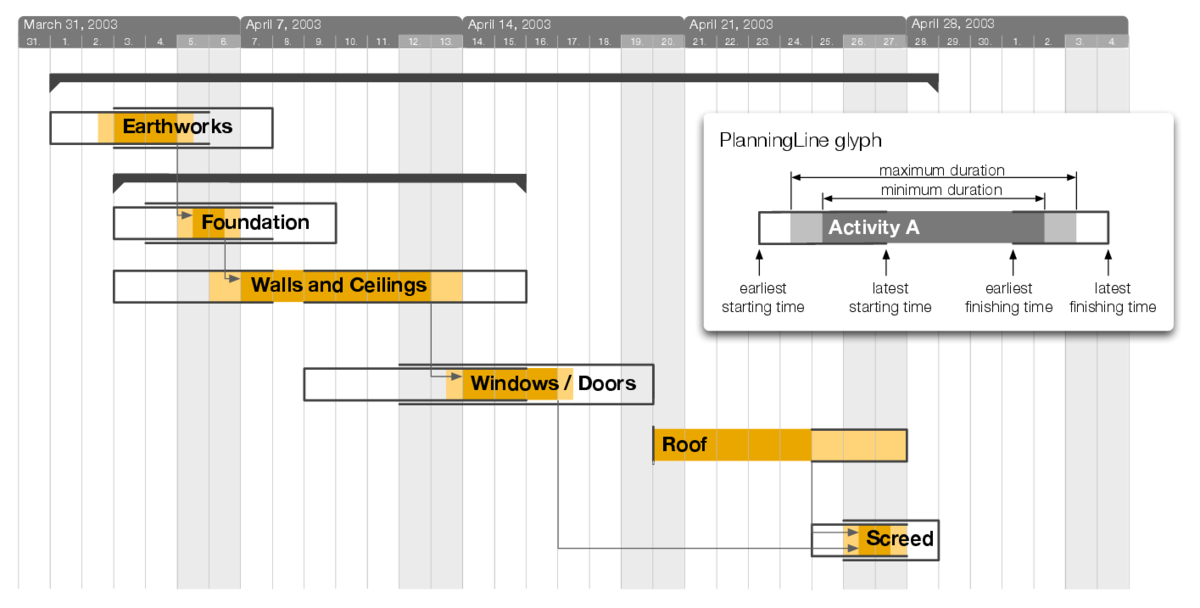
\includegraphics[width=1\linewidth]{assets/planninglines.png}
    \caption{PlannigLines \cite{aigner_planninglines_2005}}
    \label{fig:enter-label}
\end{figure}
\subsubsection{Présentation Technique}
\textbf{PlanningLines} est une technique de visualisation développée par Aigner et al. (2005) pour représenter les incertitudes temporelles dans des contextes tels que la gestion de projets ou la planification des traitements médicaux. L’objectif de PlanningLines est d’intégrer visuellement les incertitudes sur le début, la fin, et la durée des activités dans des schémas temporels traditionnels tels que les diagrammes de Gantt. Chaque PlanningLine est un glyphe qui représente les intervalles possibles pour chaque tâche : deux barres encapsulées indiquent les durées minimale et maximale, encadrées par deux "caps" (début et fin). Ce format aide à visualiser rapidement les périodes de début et de fin possibles pour chaque tâche, ce qui permet de distinguer facilement les incertitudes liées aux dates et aux durées dans une même activité \cite{aigner_planninglines_2005}.

\subsubsection{Interactions et Tâches Possibles}
Les utilisateurs peuvent interagir avec les PlanningLines pour explorer et manipuler les durées et intervalles temporels. Par exemple, le déplacement des barres de durée dans les limites définies permet de tester différentes hypothèses de planification.  Ce système permet également de visualiser la distribution de probabilité des tâches, donnant aux utilisateurs la possibilité de modéliser la variabilité des activités avec des débuts ou fins ouverts et des probabilités associées.

\subsubsection{Contraintes Matérielles}
PlanningLines nécessite une interface graphique prenant en charge des interactions fluides avec des données visuelles riches. Bien que cette technique puisse fonctionner sur des écrans standards, des écrans de grande taille et à haute résolution améliorent la lisibilité et la précision des manipulations, surtout pour des projets de grande envergure avec de nombreux intervalles \cite{aigner_planninglines_2005}.

\subsubsection{Application pour la Réservation}
Dans un système de réservation, PlanningLines pourrait être utilisé pour gérer les réservations avec des incertitudes temporelles, telles que des créneaux flexibles ou des périodes variables. Par exemple, pour des événements ou salles dont les horaires de début et de fin sont susceptibles de varier, PlanningLines permettrait de visualiser les intervalles possibles, facilitant la coordination avec d’autres créneaux et réduisant les conflits. Cette approche serait particulièrement utile dans des environnements où les réservations sont sujettes à des changements fréquents, nécessitant une flexibilité d’ajustement et une vision claire des options temporelles \cite{aigner_planninglines_2005}.

\subsection{DateLens : Interface de Calendrier Fisheye pour PDA}
\begin{figure}
    \centering
    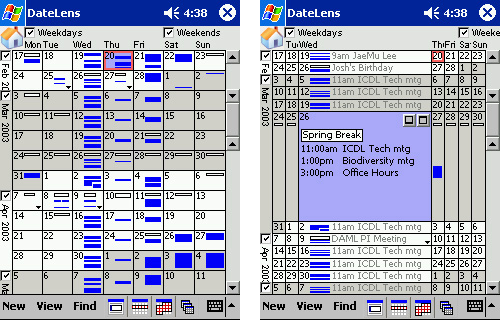
\includegraphics[width=1\linewidth]{assets/datelens.png}
    \caption{DateLens \cite{bederson_datelens_2004}}
    \label{fig:enter-label}
\end{figure}
\subsubsection{Présentation Technique}
\textbf{DateLens} est une interface de calendrier développée pour les PDA, conçue pour répondre aux défis d'affichage des informations de planification complexe sur de petits écrans. Grâce à une distorsion fisheye, elle permet aux utilisateurs de consulter des informations détaillées du calendrier tout en conservant une vue d’ensemble. DateLens utilise une structure de grille où les utilisateurs peuvent se concentrer sur des dates spécifiques, en agrandissant ou réduisant les détails dynamiquement selon les besoins. Cette approche, combinant fisheye et zoom sémantique, affiche les informations focalisées en haute définition tout en montrant le contexte avec moins de détails, optimisant ainsi l'espace limité sur les écrans des PDA \cite{bederson_datelens_2004}.

\subsubsection{Interactions et Tâches Possibles}
DateLens offre plusieurs interactions qui facilitent la gestion des plannings, notamment le zoom sur des jours, semaines ou mois spécifiques par des actions de toucher et de glisser. Les utilisateurs peuvent passer facilement d’une période à l’autre, grâce à des animations qui maintiennent l’orientation au sein du calendrier. DateLens intègre également une réglette pour contrôler les semaines visibles et des cases à cocher pour filtrer certains jours ou mois. Ces interactions permettent des tâches telles que la navigation dans des plannings complexes, la recherche d’événements et la révision de rendez-vous, offrant une vue fluide et détaillée des plannings personnels \cite{bederson_datelens_2004}.


\subsubsection{Contraintes Matérielles}
DateLens a été optimisé pour fonctionner efficacement dans les contraintes matérielles des PDA, avec des exigences modérées en termes de puissance de calcul pour le rendu et les animations. Son principal besoin est un écran haute résolution pour garantir une clarté dans l’affichage des informations détaillées. La simplicité des éléments de son interface permet une adaptation facile aux écrans plus grands, bien que les appareils de taille plus réduite, comme certains smartphones, puissent rencontrer des défis en termes d'espace d'affichage \cite{bederson_datelens_2004}.

\subsubsection{Application pour la Réservation}
Dans les systèmes de réservation, DateLens pourrait être particulièrement utile pour les utilisateurs souhaitant gérer leurs réservations personnelles ou suivre la disponibilité des ressources sur différentes périodes. Sa capacité à afficher des détails temporels contextuellement, sans surcharger l’utilisateur, le rend idéal pour des scénarios où un équilibre entre les détails immédiats et le contexte temporel plus large est nécessaire. Cela inclut la planification de salles ou de ressources sur plusieurs semaines et mois, où les utilisateurs doivent naviguer rapidement entre des perspectives détaillées et globales. La vue fisheye permet une gestion efficace des réservations sur des appareils mobiles, en répondant aux contraintes d’espace d’écran tout en offrant une interaction efficiente \cite{bederson_datelens_2004}.


\subsection{Circle View}
\begin{figure}
    \centering
    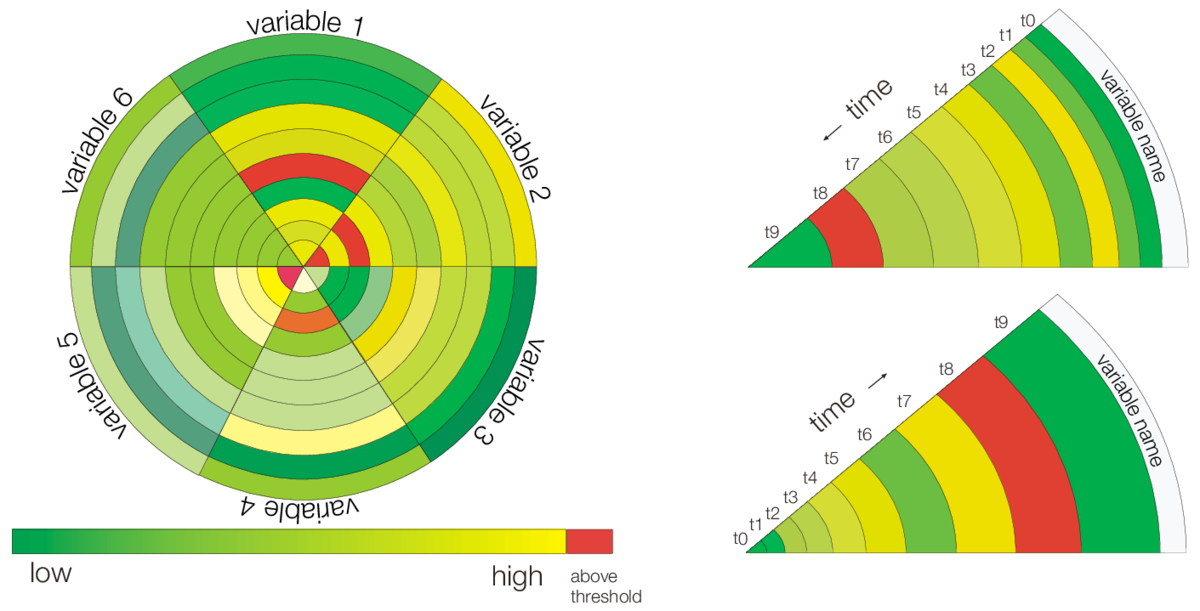
\includegraphics[width=1\linewidth]{assets/circleview.png}
    \caption{CircleView \cite{keim_circleview_2004}}
    \label{fig:enter-label}
\end{figure}
\subsubsection{Présentation Technique}
Circle View est une technique de visualisation introduite par Keim, Schneidewind, et Sips (2004) qui permet de représenter des ensembles de données temporelles et multidimensionnelles. Inspirée des treemaps et des segments de cercle, Circle View divise un cercle en plusieurs segments, chacun représentant une dimension de données. Chaque segment est ensuite subdivisé pour afficher la distribution et les changements des données au fil du temps. Cette approche permet aux utilisateurs de repérer des motifs, des exceptions et des similitudes en visualisant l'évolution des valeurs d'attributs dans un cadre circulaire, ce qui est particulièrement utile pour des analyses temporelles continues \cite{keim_circleview_2004}.

\subsubsection{Interactions et Tâches}
Circle View offre une variété d'interactions pour l'utilisateur, telles que la navigation et le filtrage des données, le drill-down pour accéder à des niveaux de détail inférieurs, ainsi que la possibilité de comparer visuellement des valeurs temporelles entre les segments adjacents. Les utilisateurs peuvent ajuster la disposition des segments et effectuer des recherches de similitudes pour mettre en évidence les corrélations dans les données temporelles. Ces interactions facilitent la découverte des schémas temporels et des relations multidimensionnelles \cite{keim_circleview_2004}.


\subsubsection{Contraintes Matérielles}
Circle View est particulièrement adapté aux écrans de grande taille et à haute résolution pour maximiser la lisibilité et faciliter la comparaison entre les segments de données. Pour les applications en temps réel, des équipements performants sont recommandés afin de garantir une mise à jour fluide des données. Cette technique fonctionne mieux sur des dispositifs capables d'afficher des informations visuelles denses \cite{keim_circleview_2004}.

\subsubsection{Application pour les Systèmes de Réservation}
Dans un système de réservation, Circle View pourrait être utilisé pour visualiser des données d'occupation et de disponibilité à travers différentes ressources et périodes. Chaque segment pourrait représenter une ressource spécifique (par exemple, des salles de réunion), et les sous-segments indiqueraient l'occupation au cours de périodes définies. Ce type de visualisation permettrait aux gestionnaires et aux utilisateurs finaux de repérer facilement les créneaux disponibles et d'anticiper les périodes de forte demande, facilitant ainsi une gestion proactive des réservations \cite{keim_circleview_2004}.


\subsection{Timeline Linéaire}
\begin{figure}
    \centering
    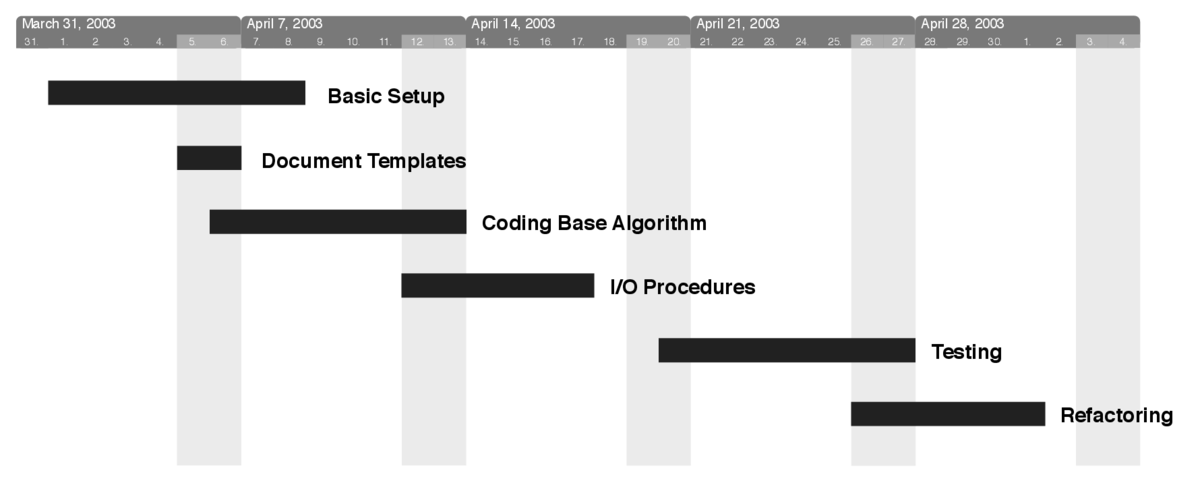
\includegraphics[width=1\linewidth]{assets/timeline_lineaire.png}
    \caption{Timeline Linéaire \cite{brehmer_timelines_2017}}
    \label{fig:enter-label}
\end{figure}

\subsubsection{Présentation Technique}
Les timelines linéaires sont l'une des méthodes les plus couramment utilisées pour visualiser des séquences d'événements dans un ordre chronologique. Ce format classique permet de mapper les événements le long d'une ligne continue, où le temps progresse horizontalement de gauche à droite. Cette approche, qui remonte au "Chart of Biography" de Joseph Priestley en 1765, est intuitive pour les utilisateurs familiarisés avec la lecture de gauche à droite. Les événements peuvent être représentés par des marqueurs, des lignes ou des icônes le long de l'axe, indiquant ainsi la séquence et la durée de chaque événement \cite{brehmer_timelines_2017}.

\subsubsection{Interactions et Tâches}
Les interactions dans les timelines linéaires incluent couramment des outils de navigation tels que le zoom et le panoramique, permettant aux utilisateurs d'ajuster leur vue pour se concentrer sur des événements ou des périodes spécifiques. Cela facilite l'examen de périodes détaillées ou la vue d'ensemble sur une timeline étendue. De nombreuses applications de timeline linéaire, telles que TimelineJS, permettent une narration interactive en permettant aux utilisateurs de cliquer sur des événements pour obtenir des informations supplémentaires. Ces interactions rendent les timelines linéaires particulièrement utiles pour l'analyse exploratoire de données et la narration d'histoires où l'ordre séquentiel et la durée des événements sont essentiels pour la compréhension de l'utilisateur \cite{brehmer_timelines_2017}.


\subsubsection{Contraintes Matérielles}
Les timelines linéaires sont polyvalentes et peuvent être utilisées efficacement sur divers types d'écrans, des appareils mobiles aux grands écrans d'ordinateur. Cependant, pour un confort d'utilisation optimal, les écrans de grande taille sont préférables car ils offrent plus d'espace pour afficher une large gamme d'événements sans chevauchement. Sur les écrans plus petits, les options interactives telles que le panoramique et le zoom sont essentielles pour maintenir la lisibilité et éviter une surcharge d'informations. Cette adaptabilité rend la timeline linéaire pratique pour les outils de visualisation aussi bien sur les ordinateurs de bureau que sur les appareils mobiles \cite{brehmer_timelines_2017}.

\subsubsection{Application pour les Systèmes de Réservation}
Dans un contexte de réservation, les timelines linéaires sont bien adaptées pour afficher les informations de réservation dans le temps, comme l'occupation des chambres d'hôtel ou la disponibilité des salles de conférence. Une vue linéaire permet aux utilisateurs de voir les schémas de réservation, d'identifier les périodes de forte demande et de repérer les chevauchements ou les créneaux disponibles. Cette approche visuelle soutient l'efficacité opérationnelle en permettant aux utilisateurs d'évaluer rapidement les créneaux ouverts et de gérer les plannings de manière efficace, facilitant ainsi la planification et l'ajustement des réservations pour les clients et les gestionnaires \cite{brehmer_timelines_2017}.

\subsection{Treemap temporel}
\begin{figure}
    \centering
    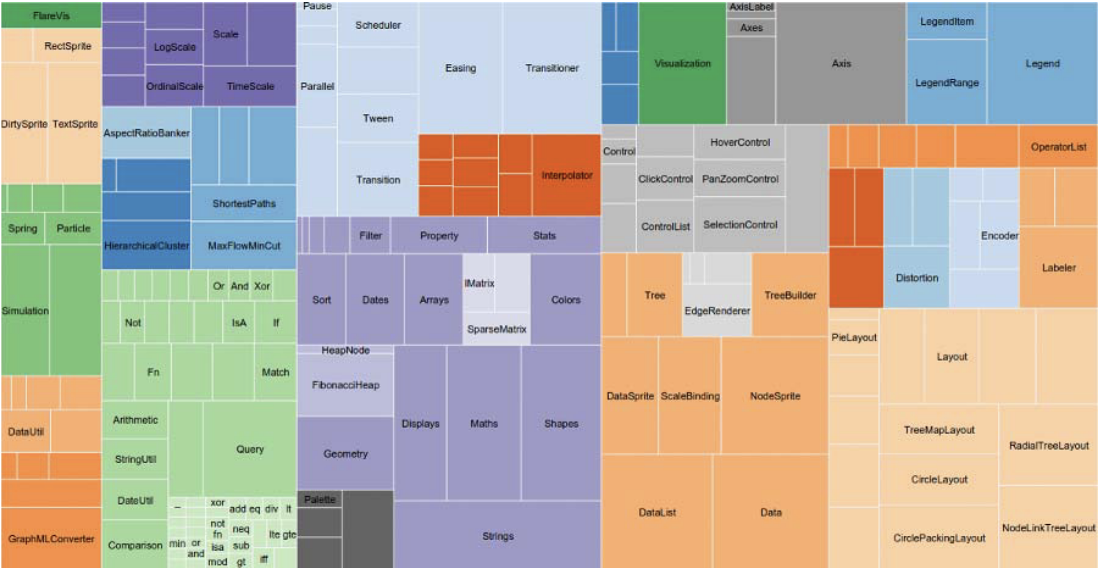
\includegraphics[width=1\linewidth]{assets/overview_treemap.png}
    \caption{Treemap \cite{figueiras_towards_2015}}
    \label{fig:enter-label}
\end{figure}
\subsubsection{Présentation technique}
Le Treemap temporel est une technique de visualisation hiérarchique qui divise l'espace en blocs proportionnels pour représenter différentes catégories de données temporelles. Chaque bloc représente une période de temps ou une activité spécifique, colorée et dimensionnée en fonction de son importance ou de sa fréquence. Cette approche hiérarchique permet d’agréger des données à des niveaux de granularité divers, offrant une vue d’ensemble tout en permettant d’accéder aux détails.

\subsubsection{Interactions et tâches possibles}
Les interactions de type drill-down sont courantes avec les Treemaps. Elles permettent aux utilisateurs de cliquer sur un bloc pour explorer une période spécifique ou un niveau de détail supérieur. De Carvalho et al. (2016) montrent que cette interaction est intuitive pour naviguer dans des périodes temporelles imbriquées, rendant l’exploration des données temporelles accessible aux utilisateurs même sans expertise technique(Daassi et al. - A taxon…).

\subsubsection{Contraintes matérielles}
Cette technique est mieux adaptée aux écrans de taille moyenne ou plus pour une visibilité optimale. Elle peut également être utilisée sur des écrans tactiles pour améliorer l’interaction par navigation.

\subsubsection{Application pour la réservation}
Le Treemap temporel est utile pour visualiser des tendances d’utilisation de ressources au fil du temps. Par exemple, dans un centre de réservation, cette technique permettrait d’identifier les périodes de forte occupation et de visualiser l’occupation de diverses salles sur plusieurs semaines ou mois.


\subsection{Perspective Wall : Technique de visualisation de l'information linéaire}
\begin{figure}
    \centering
    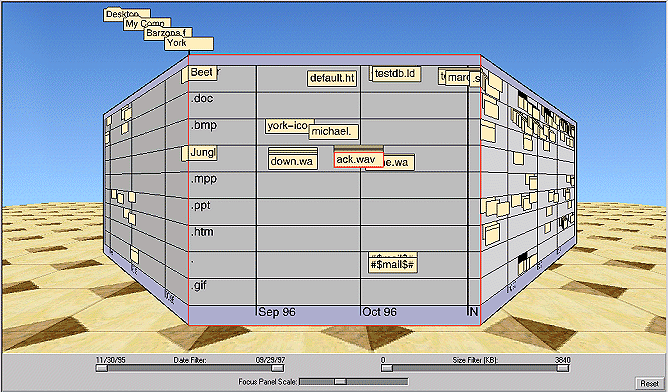
\includegraphics[width=1\linewidth]{assets/perspective-wall.png}
    \caption{Perspective Wall\cite{mackinlay_perspective_1991}}
    \label{fig:enter-label}
\end{figure}

\subsubsection{Présentation technique}
Le \textit{Perspective Wall} est une technique de visualisation développée par Mackinlay, Robertson, et Card \cite{mackinlay_perspective_1991} pour représenter des informations linéaires dans des espaces larges. Inspirée par la manière dont l'œil humain combine une vue détaillée pour le focus et une vue plus générale pour le contexte, cette technique intègre à la fois des vues de détail et des vues contextuelles dans une même interface. Le Perspective Wall "plie" visuellement une grande disposition 2D en une structure 3D, avec un panneau central dédié aux détails et deux panneaux latéraux en perspective pour le contexte. Cette structure permet une transition fluide entre les vues tout en maintenant un contexte visuel large, ce qui aide les utilisateurs à naviguer dans de vastes ensembles d'informations structurées temporellement \cite{mackinlay_perspective_1991}.

\subsubsection{Interactions et tâches possibles}
Les utilisateurs peuvent interagir avec le Perspective Wall en manipulant l’angle et la position du mur pour ajuster l'affichage. Les options d'interaction permettent de déplacer des informations du contexte vers la zone de détail en un simple glissement, offrant une vue fluide et continue sur l'ensemble de l'information. Cette interaction permet de naviguer à travers des informations linéaires tout en gardant un point de référence contextuel, essentiel pour des tâches de suivi d'événements au fil du temps, comme la visualisation de fichiers par date de modification dans un système d’information \cite{mackinlay_perspective_1991}.

\subsubsection{Contraintes matérielles}
Le Perspective Wall nécessite un support matériel pour la 3D, ce qui le rend idéal pour des stations de travail puissantes équipées de cartes graphiques capables de gérer l'animation interactive. Bien que cette technique soit adaptable sur des écrans standards, les écrans de grande taille avec haute résolution sont préférables pour maintenir la lisibilité des détails sans perte de contexte \cite{mackinlay_perspective_1991}.

\subsubsection{Application pour la réservation}
Dans un système de réservation, le Perspective Wall pourrait faciliter la gestion de créneaux horaires sur de longues périodes. Par exemple, il pourrait afficher les réservations détaillées de salles dans le panneau central tout en montrant les créneaux avant et après dans les panneaux contextuels, permettant ainsi aux utilisateurs de repérer les périodes disponibles rapidement. Cette approche permettrait une gestion proactive de la disponibilité des ressources en offrant une vue d’ensemble avec un accès rapide aux détails des créneaux de réservation \cite{mackinlay_perspective_1991}.


\subsection{Space-Time Cube (STC)}
\begin{figure}
    \centering
    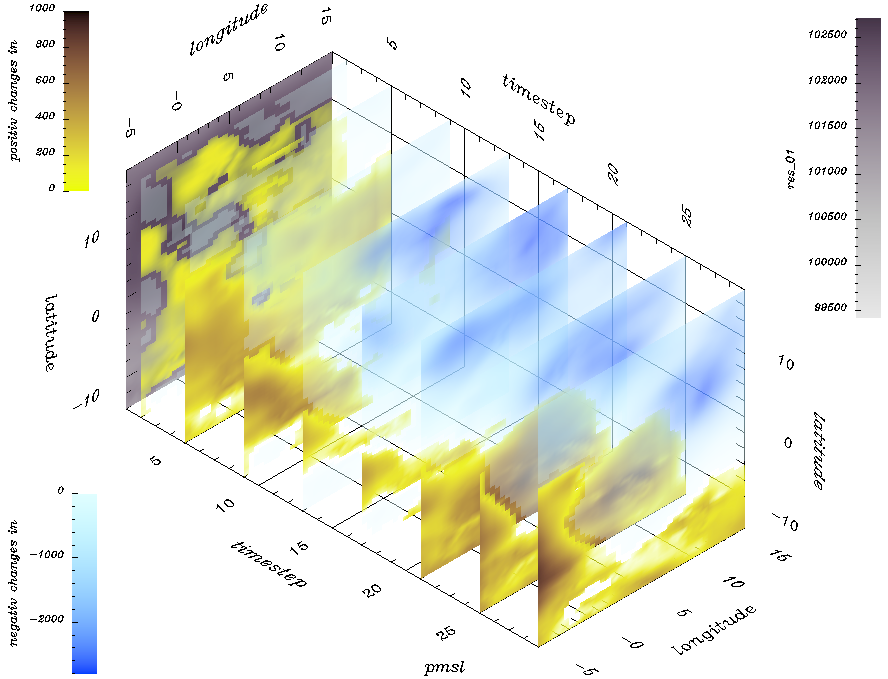
\includegraphics[width=0.75\linewidth]{assets/space-time-cube.png}
    \caption{Space Time Cube (STC) \cite{bach_review_2014}}
    \label{fig:enter-label}
\end{figure}
\subsubsection{Présentation Technique}
Le \textbf{Space-Time Cube (STC)}, introduit par Hägerstrand et développé pour la géovisualisation, est une représentation en 3D qui place l’espace sur les axes X et Y, et le temps sur l’axe Z. Cette représentation permet de suivre les trajectoires d’objets ou d’individus dans un espace donné au fil du temps, facilitant ainsi l’observation des mouvements, des stations, et des interactions spatiales et temporelles. Kraak propose une version améliorée du STC qui permet une manipulation interactive, permettant aux utilisateurs d’explorer les données sous différents angles et d’observer les trajectoires en détail, en utilisant des outils modernes de visualisation informatique \cite{bach_review_2014}.

\subsubsection{Interactions et Tâches Possibles}
Le STC permet aux utilisateurs de manipuler librement la visualisation pour observer les données sous différents points de vue. Des interactions telles que le déplacement de curseurs le long des axes permettent de sélectionner des périodes spécifiques ou des zones géographiques particulières. Les utilisateurs peuvent aussi projeter des trajectoires au sol pour visualiser les empreintes de parcours et identifier les zones de rencontre ou les périodes d’arrêt. Ces fonctions sont particulièrement utiles dans des tâches nécessitant une analyse précise des déplacements et des comportements dans le temps et l’espace \cite{bach_review_2014}.

\subsubsection{Contraintes Matérielles}
Le STC nécessite une station de travail performante pour assurer des interactions fluides, surtout avec des ensembles de données denses. La visualisation 3D peut également nécessiter un affichage de haute qualité pour éviter la surcharge visuelle. Les environnements immersifs, bien qu’offrant une meilleure perception spatiale, requièrent des casques de réalité virtuelle pour une expérience optimale, ce qui peut limiter l’accessibilité pour certains utilisateurs \cite{kraak_space-time_nodate}.

\subsubsection{Application pour la Réservation}
Dans le contexte d’un système de réservation, le STC peut être utilisé pour visualiser les schémas d’utilisation des ressources au fil du temps et dans l’espace, comme l’occupation de salles ou de ressources partagées. Il permettrait, par exemple, de voir quelles zones ou périodes sont les plus sollicitées, facilitant ainsi l’optimisation de la gestion des créneaux de réservation et la planification des ressources en fonction des schémas de fréquentation \cite{bach_review_2014}.

\subsection{Visualisation d'animation des tendances}
\begin{figure}
    \centering
    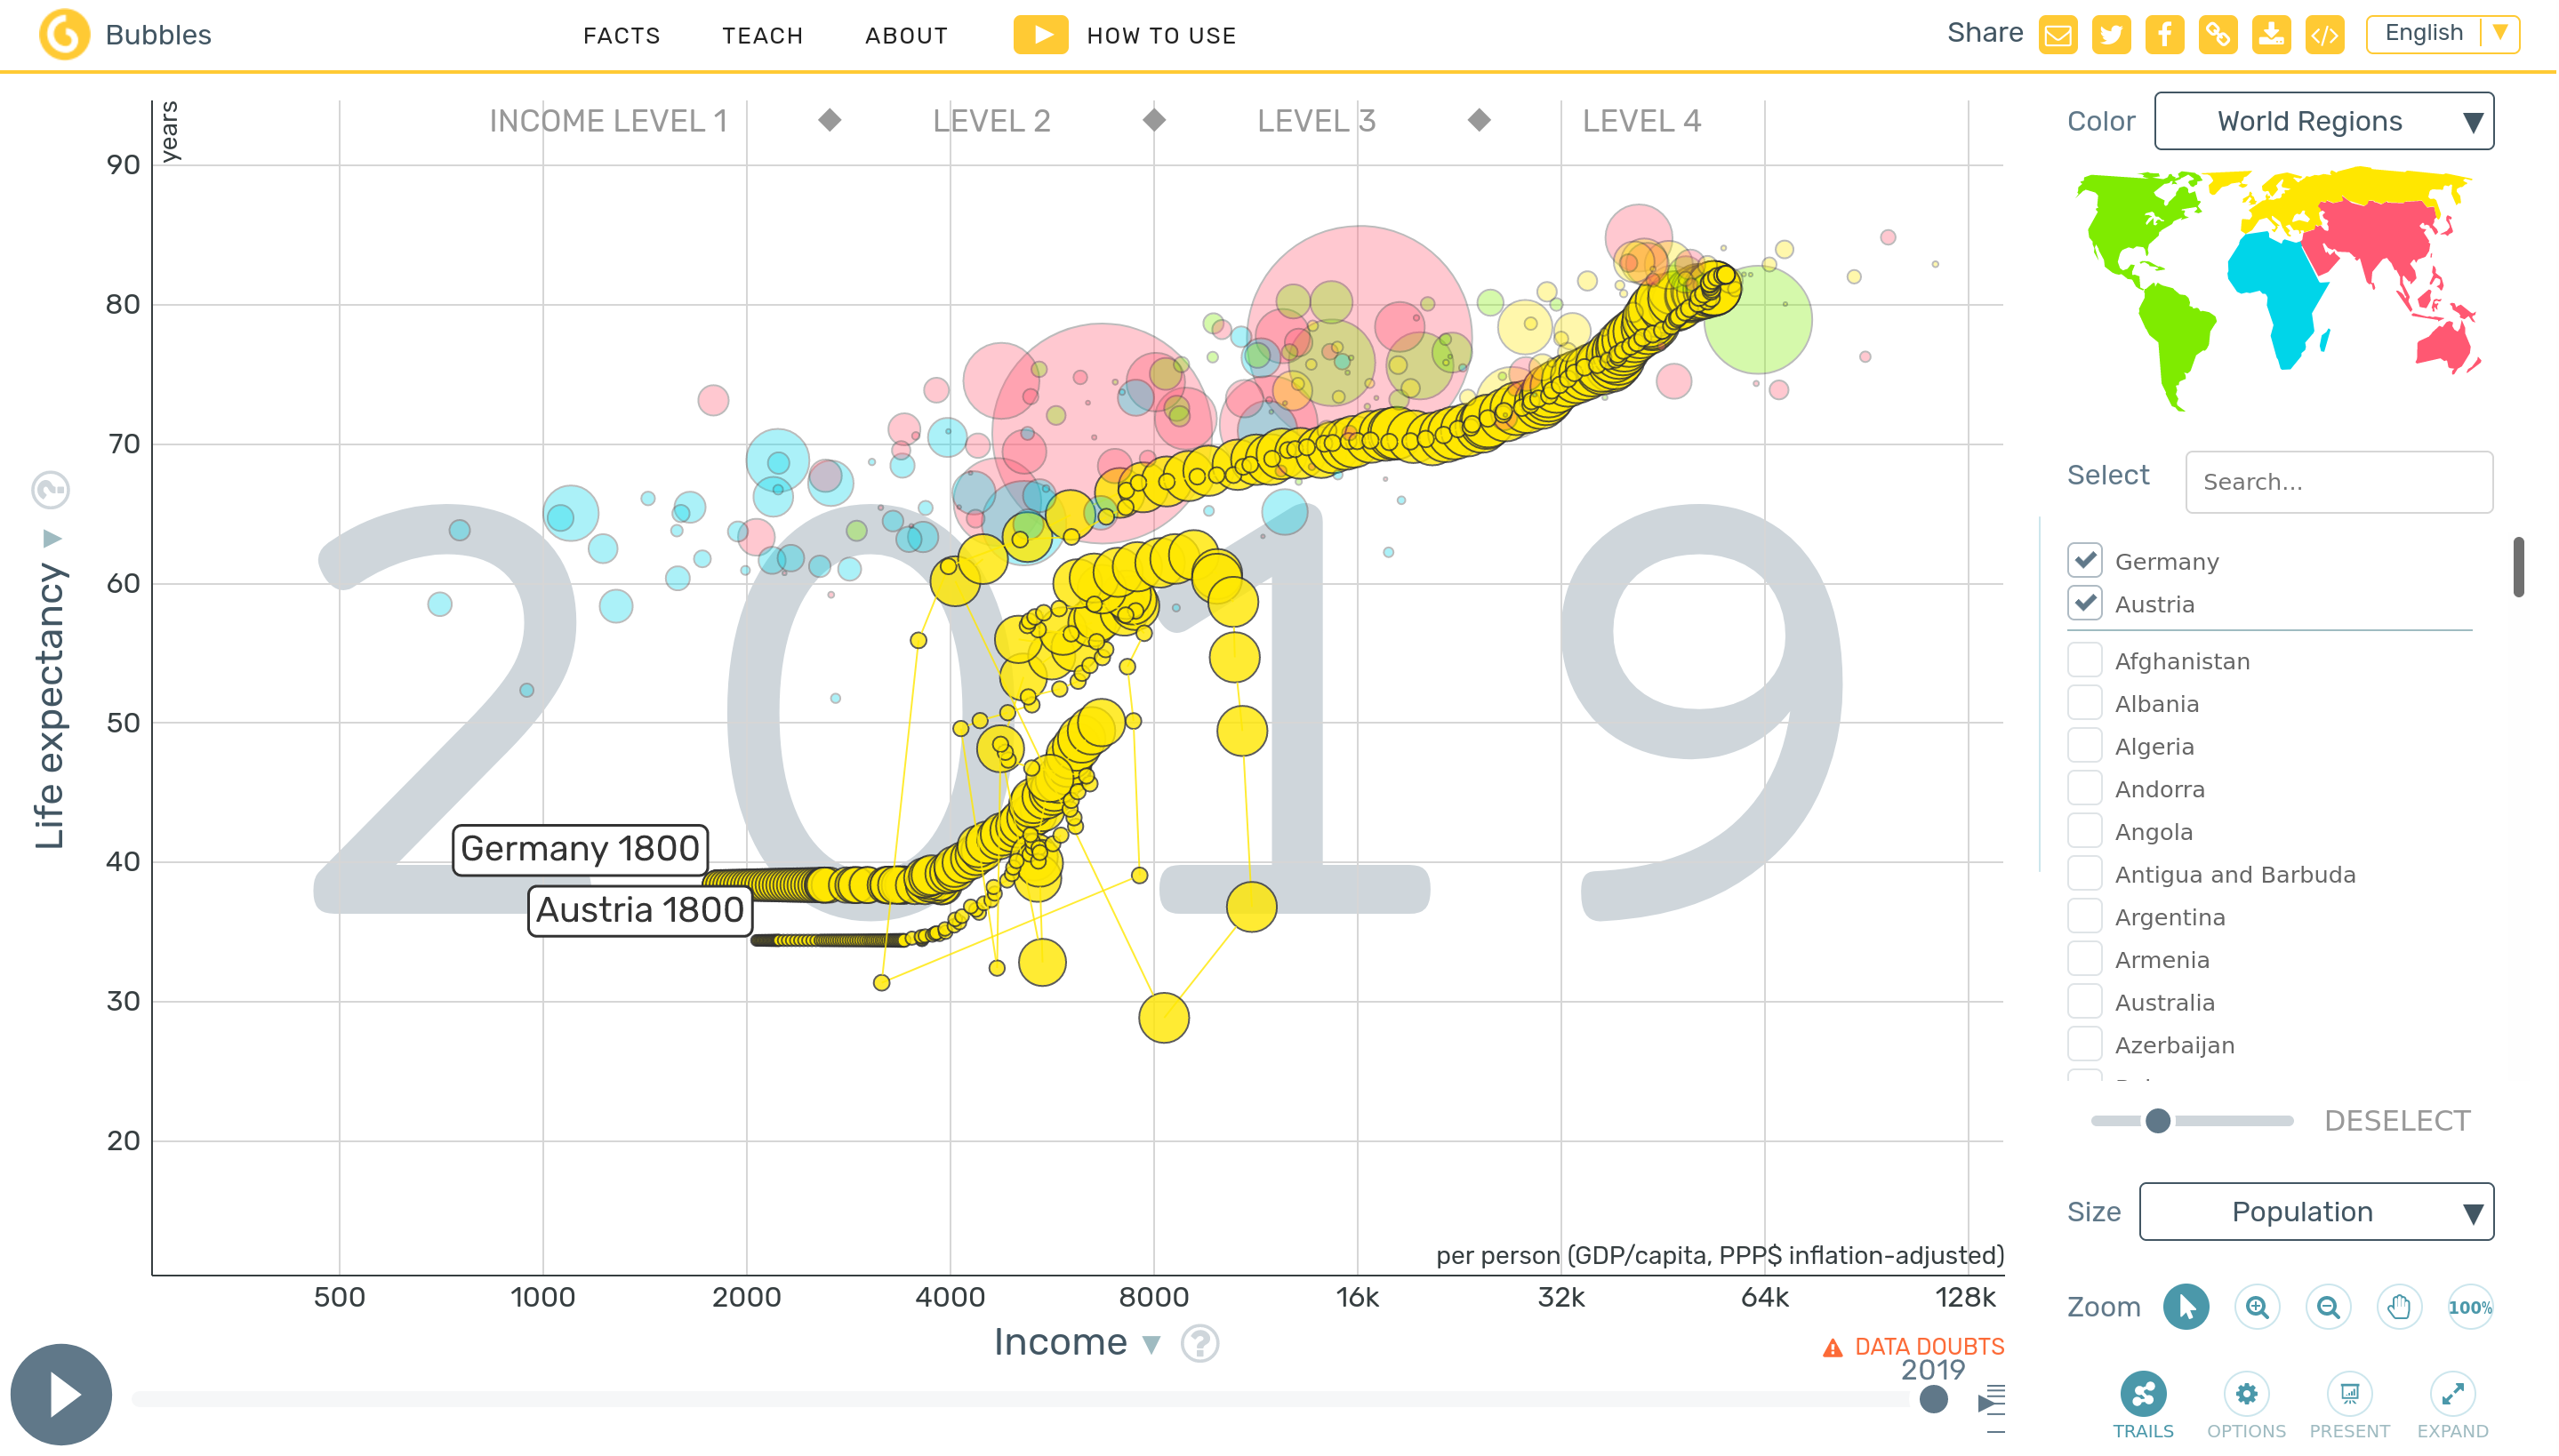
\includegraphics[width=1\linewidth]{assets/animated-scatter-plot.png}
    \caption{Animated scatter plot \cite{robertson_effectiveness_2008}}
    \label{fig:enter-label}
\end{figure}
\subsubsection{Présentation technique}  
Trendalyzer utilise un graphique à bulles animé pour représenter des données multidimensionnelles avec une dimension temporelle animée. Chaque bulle visualise des variables sur les axes X et Y, tandis que sa taille représente une troisième variable. Ce format est dynamique et permet d’illustrer la progression temporelle des tendances dans des séries de données importantes \cite{robertson_effectiveness_2008}. Pour améliorer la sélection et l'efficacité des techniques de visualisation temporelle, Aigner et al. (2023) proposent le TimeViz Browser, un outil qui catégorise diverses techniques de visualisation selon des critères simplifiés tels que la représentation visuelle (statique ou dynamique) et le type de données temporelles (linéaire ou cyclique) \cite{aigner_visualization_2023}.

\subsubsection{Interactions et tâches possibles}  
Les utilisateurs peuvent interagir avec Trendalyzer en sélectionnant des bulles spécifiques pour suivre leurs trajectoires dans le temps, tout en manipulant une barre de défilement temporel. Cette flexibilité permet de se concentrer sur des anomalies particulières ou des sous-ensembles de données. Le TimeViz Browser, quant à lui, guide les utilisateurs dans la sélection de visualisations adaptées en filtrant les techniques selon le type de temps (points ou intervalles) et la disposition (linéaire ou cyclique), simplifiant ainsi la recherche de solutions visuelles adaptées aux tâches spécifiques d’analyse de données temporelles \cite{aigner_visualization_2023}.

\subsubsection{Contraintes matérielles}  
Trendalyzer est optimisé pour des ensembles de données de taille modérée (jusqu'à 200 points), au-delà desquels les données deviennent difficilement interprétables en raison de la surcharge visuelle. TimeViz Browser aide aussi à affiner la sélection de techniques en tenant compte des dispositifs d’affichage et des modalités d’entrée, permettant ainsi de s’adapter aux contraintes matérielles telles que les petits écrans ou les interactions tactiles \cite{aigner_visualization_2023}.

\subsubsection{Application pour la réservation}  
Pour la réservation, cette technique pourrait être utilisée pour visualiser la disponibilité de ressources sur une période de temps. Les bulles animées de Trendalyzer peuvent illustrer les tendances de réservation, tandis que TimeViz Browser propose d'autres méthodes de visualisation pour des scénarios de données spatiales et temporelles en planification, comme les "Cycle Plots" pour des cycles hebdomadaires ou mensuels de réservation \cite{aigner_visualization_2023}.

\section{Conclusion [Tom]}
\subsection{Synthèse des tendances et points forts}

Parmi les tendances remarquables, on observe :

\begin{itemize}
    \item \textbf{Modularité et adaptabilité :} Certaines techniques, comme les timelines linéaires ou les histogrammes de disponibilité, se distinguent par leur simplicité et leur polyvalence. Elles conviennent aussi bien aux utilisateurs novices qu’experts, grâce à une structure qui permet une visualisation rapide des schémas temporels.
    
    \item \textbf{Support pour l’exploration de données complexes :} Des approches avancées, telles que le Space-Time Cube ou les treemaps temporels, offrent une capacité unique à représenter des données multidimensionnelles ou hiérarchiques. Elles facilitent l’analyse des relations spatiales et temporelles, ce qui peut être crucial pour les systèmes de réservation gérant des ressources multiples sur de longues périodes.
    
    \item \textbf{Interaction utilisateur enrichie :} Des techniques comme le DateLens ou le Perspective Wall intègrent des fonctionnalités interactives avancées, telles que le zoom, le panoramique ou le drill-down, qui améliorent l’exploration et l’engagement des utilisateurs. Ces interactions permettent une navigation fluide dans les données, tout en conservant une vue d’ensemble claire.
    
    \item \textbf{Visualisation de cycles et tendances :} Les graphes en spirale et les visualisations animées, comme celles de Trendalyzer, se révèlent particulièrement utiles pour identifier les cycles répétitifs et les tendances à long terme, offrant ainsi des outils stratégiques pour anticiper les périodes de forte demande.
\end{itemize}

\subsection{Défis et limitations observées}

Malgré leurs points forts, ces techniques rencontrent certaines limites qui peuvent restreindre leur adoption dans les systèmes de réservation :

\begin{itemize}
    \item \textbf{Complexité pour les utilisateurs novices :} Les méthodes avancées, telles que le Space-Time Cube ou les spirales temporelles, exigent une certaine familiarité avec les concepts de visualisation. Sans tutoriels ou interfaces simplifiées, ces techniques risquent de décourager les utilisateurs peu expérimentés.
    
    \item \textbf{Problèmes d’évolutivité :} Lorsqu'elles sont confrontées à de grands volumes de données ou à des besoins en temps réel, certaines visualisations, comme les timelines ou les treemaps, deviennent moins lisibles. Cette surcharge d’information peut nuire à la prise de décision rapide.
    
    \item \textbf{Contraintes matérielles :} Les approches exigeant une visualisation 3D, comme le Space-Time Cube, nécessitent des équipements performants, ce qui peut limiter leur accessibilité dans des contextes standards ou mobiles.
    
    \item \textbf{Surcharge cognitive :} Des techniques complexes, bien que puissantes, peuvent entraîner une surcharge cognitive pour les utilisateurs si elles ne sont pas accompagnées d’une interface bien conçue et de mécanismes de filtrage efficaces.
\end{itemize}


%
% ---- Bibliography ----
%
% BibTeX users should specify bibliography style 'splncs04'.
% References will then be sorted and formatted in the correct style.
%
% \bibliographystyle{splncs04}
% \bibliography{mybibliography}
%
\bibliographystyle{splncs04}
\bibliography{references}

\end{document}
